
In this section, we propose a unified computational account of \emph{ad hoc} coordination and convention formation that aims to address these three empirical puzzles. 
We begin from first principles: What is the core computational problem that must be solved to achieve successful communication?
Classically, this problem has been formulated in terms of coding and compression \cite{Shannon48}. 
An intended meaning in the speaker's mind must be encoded as a signal that is recoverable by the receiver after passing through a noisy transmission channel.
This literal transmission problem has since been enriched to account for \emph{pragmatics} -- the ability of speakers and listeners to use context and social knowledge to draw inferences beyond the literal meaning of messages \cite{sperber1986relevance}.
We take the Rational Speech Act framework \cite<RSA;>{frank_predicting_2012,goodman_pragmatic_2016,FrankeJager16_ProbabilisticPragmatics} as representative of this current synthesis, formalizing communication as recursive social inference in a probabilistic model.
In the next section, we will review this basic framework and then raise two fundamental computational problems facing this framework that motivate our proposal.

\subsection{RSA models of communication with static meaning}

In our referential communication setting\footnote{For concreteness, we restrict our scope to reference in a discrete context of objects, but the same formulation applies to more general spaces of meanings.}, the RSA framework defines a pragmatic speaker, denoted by $S_1$, who must choose an utterance $u$ that will allow their partner to choose a particular target object $o$ from the current communicative context $\mathcal{C}$:
They attempt to satisfy the Gricean Maxims \cite{Grice75_LogicConversation} by selecting utterances according to a utility function $U(u;o)$ that balances informativity to an imagined listener against the cost of producing an utterance.
Specifically, $S_1$ chooses from a ``softmax distribution'' concentrating mass on the utterance that maximizes $U(u;o)$ to an extent modulated by a parameter $\alpha_S \in[0,\infty]$.
As $\alpha_S \rightarrow \infty$, the speaker increasingly chooses the utterance with maximal utility.
\begin{align}
S_1(u | o) & \propto   \exp\{\alpha_S \cdot U(u; o)\}\label{eq:RSAspeaker} \\
U(u; o) & = (1-w_C) \cdot \underbrace{\log L_0(o | u)}_{\mathclap{\text{informativity}}} -\, w_C \cdot \underbrace{c(u)}_{\mathclap{\text{cost}}} \nonumber 
\end{align}
where $c(u)$ is a function giving the cost of producing $u$, assuming a longer utterances are more costly.
The speaker thus has two free parameters: $\alpha_S \in[0,\infty]$ and $w_C \in [0,1]$ which controls the relative weight of informativity and parsimony in the speaker's production.

The imagined \emph{literal listener} $L_0$ in Eq.~\ref{eq:RSAspeaker} is assumed to identify the target using a lexical meaning function $\mathcal{L}(u,o)$ capturing the literal semantics of the utterance $u$.
That is, the probability of the literal listener choosing object $o$ is proportional to the meaning of $u$ under a static lexical meaning function $\mathcal{L}$:
\begin{align}
L_0(o | u) &\propto  \mathcal{L}(u,o)\nonumber
\end{align}
Throughout this paper, we will take $\mathcal{L}$ to be a traditional truth-conditional function evaluating whether a given object is in the extension of the utterance\footnote{Note that the normalization constant may be exactly zero for some possible lexicons -- for instance, if a given utterance is literally false of all objects in context -- in which case these distributions are not well-defined. See Appendix A for technical details of how we address this problem.}:
$$
\mathcal{L}(u,o) = \left\{ \begin{array} {rl} 1 & \textrm{if $o \in \den{u}$} \\ 0 & \textrm{otherwise} \end{array}\right.
$$
However, there are many alternative representational choices compatible with our core model, including fuzzier, continuous semantics \cite{degen2020redundancy} or vector embeddings learned by a neural network \cite[see Appendix B for examples]{potts2019case}, which may be more appropriate for scaling the model to larger spaces of words and referents.
We return to these possibilities in the General Discussion.

%Finally, we may then define a pragmatic listener $L_1$ that inverts their own internal model of an imagined speaker, inferring which intended referent $o\in\mathcal{C}$ would best explain the speaker's choice of utterance $u$:
%\begin{align}
%L_1(o | u) \propto   \exp\{w_L \cdot \log S_1(u | o)\}\nonumber
%\end{align}
%Intuitively, this listener is able to account for alternative utterances the speaker could have chosen to produce.
%For example, if an alternative utterance $u'$ would have perfectly referred to some object $o$, then the fact that the speaker did \emph{not} choose to say $u'$ suggests $o$ is not the intended referent. 

\subsection{Two fundamental problems for static meaning}

This basic framework and its extensions have accounted for a variety of important phenomena in pragmatic language use \cite<e.g.>{Scontras_problang,KaoWuBergenGoodman14_NonliteralNumberWords,TesslerGoodman16_Generics,LassiterGoodman15_AdjectivalVagueness}.
Yet it retains a key assumption from classical models: that the speaker and listener must share the same literal ``protocol'' $\mathcal{L}$ for encoding and decoding messages.
In this section, we highlight two under-appreciated challenges of communication that complicate this assumption. 

The first challenge is \emph{variability} in linguistic meaning throughout a language community. 
Different listeners may recover systematically different meanings from the same message, and different speakers may encode the same message in different ways.
For example, doctors may fluently communicate with one another about medical conditions using specialized terminology that is meaningless to a patient. 
The words may not be in the patient's lexicon, and even common words may be used in non-standard ways.
That is, being fluent speakers of the same language does not ensure perfect overlap for the relevant meanings that need to be transmitted in every context: different partners may simply be using different functions $\mathcal{L}$.



The second challenge is the \emph{non-stationarity} of the world. 
Agents are continually presented with new thoughts, feelings, and entities, which they may not already have efficient conventions to talk about.
For example, when new technology is developed, the community of developers and early adopters must find ways of referring to the new concepts they are working on (e.g. \emph{e-mailing}, \emph{the Internet}). 
Or, when researchers design a new experiment with multiple conditions, they must find ways of talking about their own \emph{ad hoc} abstractions, often converging on idiosyncratic names that can be used seamlessly in meetings.
That is, any literal protocol $\mathcal{L}$ that we may write down at one time would be quickly outdated at a later time \cite<see>[for a demonstration of the related problems posed by non-stationary for large neural language models]{lazaridou2021pitfalls}.
We must have some ability to extend our language on the fly as needed.


\subsection{A hierarchical model of dynamic meaning}

%The model we present in this section aims to provide an explanation for how agents may  these fundamental problems.
Rather than assuming a monolithic, universally shared language, we argue that agents solve the core problems posed by variability and non-stationarity by attempting to continually, adaptively \emph{infer} the system of meaning used by each partner, in context.
When all agents are continually learning in this way, we will show that they are not only able to locally coordinate on \emph{ad hoc} meanings with specific partners but also able to abstract away linguistic conventions that are expected to be shared across an entire community.
We introduce our model in three steps, corresponding to three core capacities: hierarchical uncertainty about meaning, online partner-specific learning, and inductive generalization.

\paragraph{C1:~Hierarchical uncertainty about meaning} 

When an agent encounters a communication partner, they must call upon some representation about what they expect different signals will mean to that partner. 
We therefore replace the static function $\mathcal{L}$ with a \emph{parameterized family} of lexical meaning functions by $\mathcal{L}_{\phi}$, where different values of $\phi$ yield different possible systems of meaning. 
To expose the dependence on a fixed system of meaning, Eq.~\ref{eq:RSAspeaker} can be re-written to give behavior under a fixed value of $\phi$:
\begin{align}
L_0(o | u, \phi) &\propto  \mathcal{L}_\phi(u,o)\hfill\label{eq:RSA} \\
U(u; o, \phi) & = (1-w_C) \cdot \log L_0(o | u, \phi) -\, w_C \cdot c(u) \nonumber  \\
S_1(u | o,\phi) & \propto   \exp\{\alpha_S \cdot U(u; o, \phi)\} \nonumber 
%L_1(o | u,\phi) & \propto   \exp\{w_L \cdot \log S_1(u | o, \phi) \nonumber \}
\end{align}
While we will remain agnostic for now to the exact functional form of $\mathcal{L}_\phi$ and the exact parameter space of $\phi$ (see \emph{Inference details} section below), there are two computational desiderata we emphasize.

First, given the challenge of variability raised in the previous section, these expectations ought to be sensitive to the overall statistics of the population. 
An agent should know that there is tighter consensus about the meaning of \emph{dog} than the meaning of, say, specialized medical terms like \emph{sclerotic aorta} \cite{Clark98_CommunalLexicons}, and conversely, should expect more consensus around how to refer to familiar concepts than new or ambiguous concepts.
This desideratum -- representing population variability -- motivates a \emph{probabilistic} formulation.
Instead of holding a single static function $\mathcal{L}_{\phi}$, which an agent assumes is shared perfectly in common ground (i.e. one $\phi$ for the whole population), we assume each agent maintains \emph{uncertainty} over the exact meaning of words as used by different partners.
In a Bayesian framework, this uncertainty is specified by a prior probability distribution over possible values of $\phi$.
For example, imagine that under some possible values of $\phi$, the term ``sclerotic aorta'' has truth conditions related to a specific condition of the heart, but under other values of $\phi$, it does not: a well-trained doctor approaching a stranger should not assume their partner is using either $\phi$ but should assign some probability to each case.
The introduction of uncertainty over a partner's literal semantics has previously been explored in the context of one-shot pragmatic reasoning, where it was termed \emph{lexical uncertainty} \cite{bergen_pragmatic_2016}, and in the context of iterated dyadic interactions \cite{SmithGoodmanFrank13_RecursivePragmaticReasoningNIPS}. 

\begin{figure}[b!]
\centering
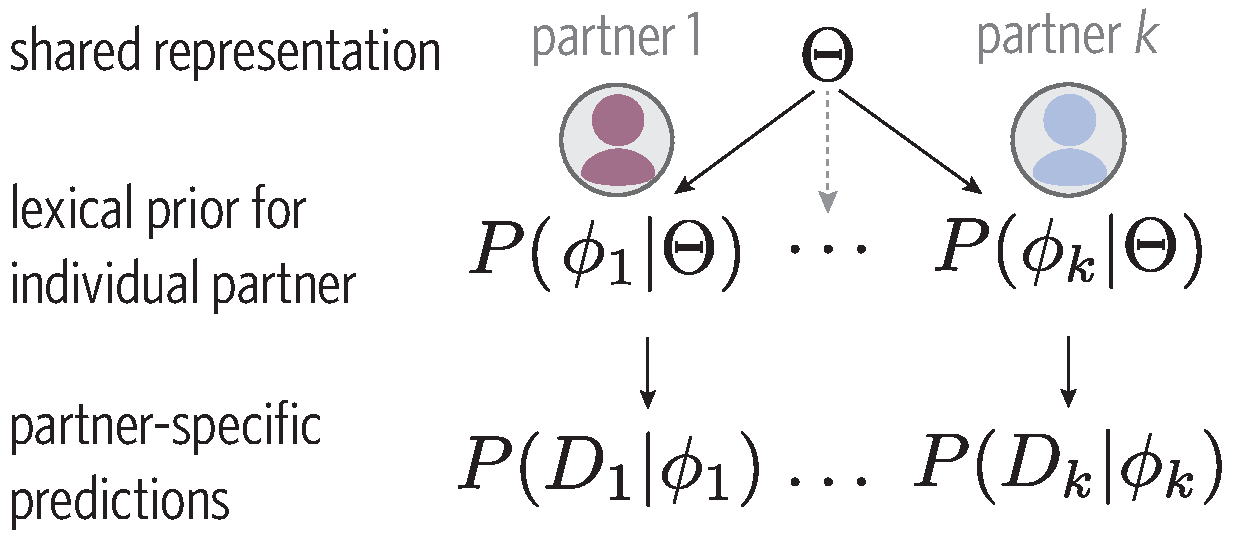
\includegraphics[scale=0.35]{./figures/task1_model.pdf}
\vspace{.5em}
\caption{\emph{Schematic of hierarchical Bayesian model.} At the highest level, denoted by $\Theta$, is a representation of aspects of meanings expected to be shared across all partners. These \emph{global} conventions serve as a prior for the systems of meanings used by specific partners, $\phi_k$. These partner-specific representations give rise in turn to predictions about their language use $P(D_k|\phi_k)$, where $D_k$ represents observations in a communicative interaction with partner $k$. By inverting this model, agents can adapt to \emph{local} partner-specific conventions and update their beliefs about global conventions.}
\label{fig:model_schematic}
\end{figure}

Second, this representation should also, in principle, be sensitive to the social identity of the partner: a cardiologist should have different expectations about a long-time colleague than a new patient.
This desideratum -- sensitivity to partner-specific meanings -- motivates a \emph{hierarchical} model, where uncertainty is represented by a multi-level prior. 
At the highest level of the hierarchy is \emph{community-level} uncertainty $P(\Theta)$, where $\Theta$ represents an abstract ``overhypothesis'' about the overall distribution of possible partners. 
$\Theta$ then parameterizes the agent's \emph{partner-specific} uncertainty $P(\phi_{k} | \Theta)$, where $\phi_k$ represents the specific system of meaning used by partner $k$ (see Fig. \ref{fig:model_schematic}). 
We focus for simplicity on this basic two-layer hierarchy, but the model can be straightforwardly extended to representing uncertainty at intermediate layers of social structure, including whether partners belong to distinct sub-communities (e.g. represented by discrete latent variables) or varying along latent dimensions (e.g. represented by a topic mixture). 
We return to these possible extensions in the General Discussion.

To integrate lexical uncertainty into our speaker and listener models, we assume they each act in a way that is expected to be successful \emph{on average}, under likely values of $\phi_k$ \cite{SmithGoodmanFrank13_RecursivePragmaticReasoningNIPS}.
In other words, they sample actions by marginalizing over their own beliefs $P_S(\phi_k)$ or $P_L(\phi_k)$ about different meanings their partner $k$ may be using.
\begin{align}
L(o|u) &\propto   \exp\left\{\alpha_L\cdot \textstyle{\int} P_L(\phi_k)  \log S_1(u|o, \phi_k)\,\,d\phi_k\right\}\nonumber\\
S(u|o) &\propto  \exp\left\{\alpha_S \cdot \textstyle{\int} P_S(\phi_k)  U(u; o, \phi_k) \,\,d\phi_k\right\}\label{eq:marginalized}
\end{align}
where $\alpha_S, \alpha_L \in[0,\infty]$ control the speaker's and listener's soft-max optimality, respectively\footnote{We denote $L$ and $S$ without a subscript because they are the only speaker and listener models we use in simulations throughout the paper -- the subscripted definitions are internal constructs used to define these models -- but in the terminology of the RSA framework they represent $L_1$- and $S_1$-level pragmatic agents with lexical uncertainty. We found that higher levels of recursion were not strictly necessary to derive the phenomena of interest, but $L_n$ and $S_n$-level lexical uncertainty models may be generalized by replacing $S_1$ in the listener equation, and $L_0$ in the speaker's utility definition, with standard RSA definitions of $n-1$-level agents \cite<e.g.>{zaslavsky2020rate}.}.

\paragraph{C2: Partner-specific online learning}

The formulation in Eq.~\ref{eq:marginalized} derives how agents ought to act under uncertainty about the lexicon being used by their partner, $P(\phi_k)$.
But how do beliefs about their partner change over time?
Although an agent may begin with significant uncertainty about the system of meaning their partner is using in the current context, further interactions provide useful information for reducing that uncertainty and therefore improving the success of communication.
In other words, \emph{ad hoc} convention formation may be re-cast as an inference problem.
Given observations $D_k$ from interactions with partner $k$, an agent can update their beliefs about their partner's latent system of meaning following Bayes rule:
\begin{equation}
\begin{array}{rcl}
\label{eq:joint_inference}
P(\phi_k, \Theta | D_k)  & \propto &  P(D_k | \phi_k, \Theta) P(\phi_k, \Theta) \\
                           & =   & P(D_k | \phi_k) P(\phi_k | \Theta) P(\Theta)
\end{array}
\end{equation}
This joint inference decomposes the partner-specific learning problem into two terms, a prior term $P(\phi_k | \Theta)P(\Theta)$ and a likelihood term $P(D_k | \phi_k)$.
The prior term captures the idea that, in the absence of strong evidence of partner-specific language use, the agent ought to regularize toward their background knowledge of conventions: the aspects of meaning that all partners are expected to share in common.
The likelihood term represents predictions about how a partner would use language in context under different underlying systems of meaning (as specified in the \emph{Referential Feedback} section below).

Importantly, the posterior obtained in Eq.~\ref{eq:joint_inference} allows agents to explicitly maintain \emph{partner-specific expectations}, as used in Eq.~\ref{eq:marginalized}, by marginalizing over community-level uncertainty:
\begin{equation}
P(\phi_k | D_k) =  \int_{\Theta}P(\phi_k, \Theta | D_k)  d\Theta
\end{equation}
This posterior can be viewed as the ``idiolect'' that has been fine-tuned to account for partner-specific common ground from previous interactions.
We will show that when agents learn about their partner in this way, and adjust their own production or comprehension accordingly (i.e.~Eq.~\ref{eq:marginalized}), they are able to coordinate on stable \emph{ad hoc} conventions.

\paragraph{C3: Inductive generalization to new partners}

The posterior in Eq.~\ref{eq:joint_inference} also provides an inductive pathway for partner-specific data to inform beliefs about community-wide conventions.
Agents update their beliefs about $\Theta$, using data accumulated from different partners, by marginalizing over beliefs about specific partners:
\begin{equation}
\begin{split}
    P(\Theta | D)  = & \int_{\phi} P(\phi, \Theta | D) d\phi \\
%                     \propto & P(\Theta) \int_{\phi} P(D_k | \phi_k) P(\phi_k | \Theta) d\phi
\end{split}
\end{equation}
where $D = \bigcup_{k=1}^N D_k$, $\phi = \phi_1 \times \dots \times \phi_N$, and $N$ is the number of partners previous encountered. 
Intuitively, when multiple partners are inferred to use similar systems of meaning, beliefs about $\Theta$ shift to represent this abstracted knowledge: it becomes more likely that a novel partner in one's community will share it as well.
Note that this population-level posterior over $\Theta$ not only represents what the agent has learned about the central tendency of the group's conventions, but also the \emph{spread} or variability, capturing the notion that some word meanings may be more widespread than others.

The updated $\Theta$ should be used to guide the prior expectations an agent brings into a subsequent interactions with strangers.
This transfer is sometimes referred to as ``sharing of strength'' or ``partial pooling'' because pooled data is smoothly integrated with domain-specific knowledge.
This property has been key to explaining how the human mind solves a range of other difficult inductive problems in the domains of concept learning \cite{KempPerforsTenenbaum07_HBM, tenenbaum_how_2011}, causal learning \cite{KempPerforsTenenbaum07_HBM,KempGoodmanTenenbaum10_LearningToLearn},  motor control \cite{berniker2008estimating}, and speech perception \cite{kleinschmidt2015robust}.
A key consequence of such transfer hierarchical models is the ``blessing of abstraction,'' \cite{GoodmanUllmanTenenbaum11_TheoryOfCausality} where it is possible under certain conditions for beliefs about the community's conventions \emph{in general} to outpace beliefs about the idiosyncracies of individual partners \cite{gershman2017blessing}.
We return to this property in the context of language acquisition in the General Discussion.

\subsection{Further challenges for convention formation}

The formulation in the previous section presents the core of our theory.
Here, we highlight several additional features of our model, which address more specific challenges raised by prior work on communication and which we will encounter in the simulations reported in the remainder of the paper. 
Our organization of these details is motivated by the analysis of \citeA{spike_minimal_2017}, who recently distilled three common problems that all accounts of convention must address: (1) the availability of referential feedback, (2) a form of information loss or forgetting, and (3) a systemic bias against ambiguity.
Finally, we explain practical details of how we perform inference in this model. 

\paragraph{Referential feedback}

Learning and adaptation depends on the availability and quality of observations $D_k$ throughout a communicative interaction.
If the speaker has no way of assessing the listener's understanding, or if the listener has no way of comparing their interpretation against the speakers intentions, however indirectly, they can only continue to rely on their prior, with no ground for conventions to form  \cite{KraussWeinheimer66_Tangrams,HupetChantraine92_CollaborationOrRepitition,GarrodFayLeeOberlanderMacLeod07_GraphicalSymbolSystems}.
So, what data $D_k$ should each agent use to update their beliefs at a particular point in an interaction?

In principle, we expect that $D_k$ reflects all relevant sources of information that may expose an agent's understanding or misunderstanding, including verbal and non-verbal backchannels (\emph{mmhmm}, nodding), clarification questions, and actions taken in the world.
In the more minimal setting of a reference game, we use the full feedback provided by the task, where the speaker's intended target and the listener's response are revealed at the end of each trial. 
Formally, this information can be written as a set of tuples $D_k = \{o^*, u', o'\}_{t=1}^T$, where $o^*$ denotes the speaker's intended target, $u'$ denotes the utterance they produced, and $o'$ denotes the listener's response, on each previous trial $t$.

Now, to specify the likelihoods in Eq.~\ref{eq:joint_inference} for our referential setting, we assume each agent should infer their partner's lexicon $\phi_k$ by conditioning on their \emph{partner's} previous choices.
The listener on a given trial should use the probability that a speaker would produce $u$ to refer to the target $o^*$ under different $\phi_k$, i.e. $P_L(\{o^*, u', o'\}_t\, | \, \phi_k) = S_1(u'_t \,|\, o^*_t, \phi_k)$, and the speaker should likewise use the probability that their partner would produce response $o'$ after hearing utterance $u$, $P_S(\{o^*, u', o'\}_t \,|\, \phi_k) = L_0(o'_t \,|\, u'_t)$,
This symmetry, where each agent is attempting to learn from the other's behavior, creates a clear coordination problem\footnote{In some settings, agents in one role may be expected to take on more of the burden of adaptation, leading to an asymmetric division of labor \cite<e.g.>{MorenoBaggio14_AsymmetrySignaling}. This may be especially relevant in the presence of asymmetries in power, status, or capability. In principle, this could be reflected in differing values of parameters $\alpha_S$ and $\alpha_L$, but we leave consideration of such asymmetries for future work.}.
In the case of an error, where the agent in the listener role hears the utterance $u'$ and chooses an object $o'$ other than the intended target $o^*$, they will receive feedback about the intended target and subsequently condition on the fact that the speaker chose $u'$ to convey that target.
Meanwhile, the agent in the speaker role will subsequently condition on the likelihood that the listener chose the object $o'$ upon hearing their utterance.
In other words, each agent will subsequently condition on slightly different data leading to conflicting beliefs.
Whether or not agents are able to resolve early misunderstandings through further interaction and eventually reach consensus depends on a number of factors.

\paragraph{Memory and forgetting}

One important constraint is imposed by the basis cognitive mechanisms of memory and forgetting.
It is unrealistic to expect that memories of every example of every past interaction in the set of observations $D$ is equally accessible to the agent.
Furthermore, this may be to the agent's advantage.
Without any mechanism for forgetting, early errors may prevent coordination much later in an interaction, as each agent's lexical beliefs must explain all previous observations equally.
Without the ability to discount earlier data points, agents may be prevented from ever reaching consensus with their partner \cite{spike_minimal_2017}.

Forgetting is typically incorporated into Bayesian models with a decay term in the likelihood function \cite{anderson2000adaptive,angela2009sequential,fudenberg2014recency,kalm2018visual}.
$$P(D_k | \phi_k) = \prod_{\tau=0}^T \beta^{\tau} P(\{o^*,u',o'\}_{T-\tau}\, |\, \phi_k)$$
where $\tau=0$ indexes the most recent trial $T$ and decay increases further back through time.
This decay term is motivated by the empirical power function of forgetting \cite{wixted1991form}, and can be interpreted as the expectation over a process where observations have some probability of dropping out of memory at each time step.
Indeed, this likelihood can be derived by simply extending our hierarchical model down an additional layer \emph{within} each partner to allow for the possibility that they are using slightly different lexicons at different points in time; assuming a degree of auto-correlation between neighboring time points yields this form of discounting.
Alternatively, at the algorithmic level, decay can be viewed as a form of weighted importance sampling, where more recent observations are preferentially sampled \cite{pearl2010online}\footnote{While this simple decay model is sufficient for our simulations, it is missing important mechanistic distinctions between working memory and long-term memory; for example, explaining convention formation over longer timescales may require an explicit model of consolidation or source memory for context.}

\paragraph{Bias against ambiguity}

A third specific challenge is posed by ambiguity: if a speaker uses a label to refer to one target, it is consistent with the data for the listener to subsequently believe that the same expression may be acceptable for other targets as well. 
%How do agents overcome this ambiguity to converge on an \emph{informative} communication system?
In our account, this problem is naturally solved by the principles of \textit{pragmatic reasoning} instantiated in the RSA framework \cite{Grice75_LogicConversation}, which has been explicitly linked to \emph{mutual exclusivity} in word learning \cite{bloom2002children,FrankGoodmanTenenbaum09_Wurwur,SmithGoodmanFrank13_RecursivePragmaticReasoningNIPS,gulordava2020one,ohmerreinforcement}.
Gricean pragmatic reasoning critically allows agents to learn from the \emph{absence} of evidence by reasoning about alternatives. 

Pragmatic reasoning plays two distinct roles in our model.
First, Gricean agents assume that their partner is using language in a cooperative manner and account for this when inferring their partner's language model.
That is, we use these equations as the linking function in the likelihood $P(D_k | \phi_k)$, representing an agent's prediction about how a partner with meaning function $\phi_k$ would actually behave in context (Eq.~\ref{eq:joint_inference}). 
$S_1$ is used to learn from observations generated in the speaker role and $L_1$ is used to learn from observations generated in the listener role.
For example, upon hearing their partner use a particular utterance $u$ to refer to an object $o$, a pragmatic agent can not only infer that $u$ means $o$ in their partner's lexicon, but also that all other utterances $u'$ likely do \emph{not} mean $o$: if they did, the speaker would have used them instead.
Second, agents do not only make passive inferences from observation, they participate in the interaction by \emph{using language} themselves.
A Gricean agent's own production and comprehension is also guided by cooperative principles (Eq.~\ref{eq:marginalized}).

Many minor variations on the basic RSA model have been explored in previous work, and it is worth highlighting three technical choices in our formulation.
First, both agents are ``action-oriented,'' in the sense that they behave proportional to the utility of different actions, according to a soft-max normalization $\sigma(U(z)) = e^{U(z)}/\sum e^{U(z)}$.
This contrasts with some RSA applications, where the listener is instead assumed to be ``belief-oriented,'' simply inferring the speaker's intended meaning without producing any action of their own \cite{qing2015variations}.
Second, our instantiation of lexical uncertainty differs subtly from the one used by \citeA{bergen_pragmatic_2016}, which placed the integral over lexical uncertainty at a \emph{single} level of recursion (specifically, within a pragmatic listener agent).
Instead, we argue that it is more natural in an interactive, multi-agent setting for each agent to maintain uncertainty at the highest level, such that each agent is reasoning about their \emph{partner}'s lexicon regardless of what role they are currently playing.

Lastly, we must define how the $L_0$ agent behaves when an utterance is false of all objects in context under their lexicon (i.e. when the normalization constant is exactly 0). 
Previous proposals have assumed that the $L_0$ should choose uniformly in this case.
However, this assumption has the unintuitive consequence that $S_1$'s utility of using an utterance known to be false of the target may be the same as an utterance known to be true.
To address this concern, we always add a low-prior-probability `null object' to the $L_0$'s context, for which all utterances evaluate to true.
This alternative can be interpreted as a `failure to refer' and effectively prevents $L_0$ from assigning belief to a referent for which the utterance is literally false (this case is distinct from the case of a \emph{contradiction}, which arises when defining the meaning of multi-word utterances in Section \textbf{P1} below.)
See Appendix A for further details and discussion of our RSA implementation.

\paragraph{Inference details}

While our simulations in the remainder of the paper each address different scenarios, we have aimed to hold as many details as possible constant throughout the paper.
First, we must be concrete about the space of possible lexicons that parameterizes the lexical meaning function, $\mathcal{L}_{\phi}$.
For consistency with previous Bayesian models of word learning \cite<e.g.>{XuTenenbaum07_WordLearningBayesian} we take the space of possible meanings for an utterance to be the set of nodes in a concept taxonomy.
When targets of reference are conceptually distinct, as typically assumed in signaling games, the target space of utterance meanings reduces to the discrete space of individual objects, i.e.~$\den{u}_{\phi} = \phi(u) \in \mathcal{O}$ for all $u\in\mathcal{U}$.
For this special case, the parameter space contains exactly $|\mathcal{O}| \times |\mathcal{U}|$ possible values for $\phi$, corresponding to all possible mappings between utterances and individual objects. 
Each possible lexicon can therefore be written as a binary matrix where the rows correspond to utterances, and each row contains one object.
The truth-conditional function $\mathcal{L}_{\phi}(u,o)$ then simply checks whether the element in row $u$ matches object $o$.
For example, there are four possible lexicons for two utterances and two objects:
$$\phi \in \left\{\begin{bmatrix}
\bluesquare \\
\orangecircle \\
\end{bmatrix},
\begin{bmatrix}
\orangecircle \\
\bluesquare \\
\end{bmatrix},
\begin{bmatrix}
\orangecircle\\
\orangecircle \\
\end{bmatrix},
\begin{bmatrix}
\bluesquare  \\
\bluesquare \\
\end{bmatrix}\right\}$$

Second, having defined the support of the parameter $\phi$, we can then define a simplicity prior $P(\phi) \propto \exp\{-|\phi|\}$ following \citeA{FrankGoodmanTenenbaum09_Wurwur}, where $|\phi|$ is the total size of each word's extension, summed across words in the vocabulary. 
Again, for traditional signaling games, this reduces to a uniform prior because all possible lexicons are the same size: $\phi(u_i) \sim \textrm{Unif}(\mathcal{O})$.
We can compactly write distributions over $\phi$ in terms of the same utterance-object matrix, where row $i$ represents the marginal distribution over possible meanings of utterance $u_i$.
For example, the uninformative prior for two utterances and two objects can be written:
$$P(\phi) =  \begin{array}{ccc}
& & \bluesquare \,\,\,\,\,\,\orangecircle \\
\begin{bmatrix}
\textrm{Unif}\{\bluesquare,\orangecircle\} \\
\textrm{Unif}\{\bluesquare,\orangecircle\} \\
\end{bmatrix} & = & \begin{bmatrix}
.5 & .5  \\
.5 & .5 \\
\end{bmatrix}
\end{array}$$
This prior becomes more important for \textbf{P3}, however, where we consider spaces of referents with more complex conceptual structure and a larger space of possible meanings. 
A single word may apply to multiple conceptually related referents or, conversely, may have an empty meaning, where it is effectively removed from the agent's vocabulary.
In this more general case, a simplicity prior generically favors smaller word meanings as well as a smaller effective vocabulary size, since the null meaning has the smallest extension. 

Finally, while the probabilistic model we have formulated in this section is theoretically well-motivated and mathematically well-defined, it has previously been challenging to actually derive predictions from it.
Historically, interactive models have been challenging to study with closed-form analytical techniques and computationally expensive to study through simulation, likely contributing to the prevalence of simplified heuristics in prior work. 
Our work has been facilitated by recent advances in probabilistic inference techniques that have helped to overcome these obstacles. 
We have implemented our simulations in the probabilistic programming language WebPPL \cite{GoodmanStuhlmuller14_DIPPL}.
All of our simulations iterate the following trial-level loop: (1) sample an utterance from the speaker's distribution, given the target object, (2) sample an object from the listener's object distribution, given the utterance produced by the speaker, (3) append the results to the list of observations, and (4) update both agents' posteriors, conditioning on these observations before continuing to the next trial.

To obtain the speaker and listener distributions (steps 1-2; Eq.~\ref{eq:RSA}), we always use exhaustive enumeration for exact inference.
We would prefer to use enumeration to obtain posteriors over lexical meanings as well (step 4; Eq.~\ref{eq:joint_inference}), but as the space of possible lexicons $\phi$ grows, enumeration becomes intractable.
For simulations related to \textbf{P2} and \textbf{P3}, we therefore switch to Markov Chain Monte Carlo (MCMC) methods to obtain samples from each agent's posteriors, and approximate the expectations in Eq.~\ref{eq:marginalized} by summing over these samples. 
Because we are emphasizing a set of phenomena where our model makes qualitatively different predictions than previous models, our goal in this paper is to illustrate and evaluate these \emph{qualitative} predictions rather than provide exact quantitative fits to empirical data.
As such, we proceed by examining predictions for a regime of parameter values ($w_S, w_L, w_C,\beta$) that help distinguish our predictions from other accounts.
